\documentclass[10pt,twoside,a4paper]{article}
\usepackage[T1]{fontenc}
\usepackage[utf8]{inputenc}
\usepackage[portuges]{babel}
\usepackage[a4paper]{geometry}
\geometry{tmargin=1.2cm,bmargin=1.7cm,lmargin=1.5cm,rmargin=1.5cm}
\usepackage{graphicx}
\usepackage{indentfirst}
\usepackage{uniforTitle}

% Fonte similar à Arial
\usepackage{helvet}
\renewcommand{\familydefault}{\sfdefault}


%===========================
% VARIÁVEIS DO DOCUMENTO
%===========================
\evento{Ciência de Dados Aplicada à Ciência da Cidade}
\date{novembro de 2026}

\title{Além dos quilômetros: conectividade da rede cicloviária de Fortaleza}

\author[1]{Sara Pessoa\thanks{Estudante de Mestrado, email: sarapessoa.dev@gmail.com}}

\affil[1]{Universidade de Fortaleza -- Programa de Pós-Graduação em Informática Aplicada}

\keywords{Redes espaciais. Componentes conectados. Infraestrutura cicloviária. Fortaleza.}


\begin{document}
\inserirtitulo
\linespread{1.5}% Espaçamento 1.5 (como no word)

%==================================
% RESUMO
%==================================
\section{Resumo}
A extensão da malha cicloviária é o indicador mais divulgado, mas não informa se os trechos estão ligados entre si. Representamos as ciclovias e ciclofaixas de Fortaleza, a partir de dados públicos, como um grafo e calculamos seus componentes conectados. Os 429~km analisados formam 44 componentes. O maior reúne 241~km (56\% da rede), e outros dois conjuntos, a oeste e a sudeste, somam 131~km sem ligação com ele. O resultado varia pouco com a tolerância usada para unir trechos próximos e se mantém após a conferência, em imagens de satélite, das conexões incertas.

%==================================
% INTRODUÇÃO
%==================================
\section{Introdução}
Fortaleza ampliou sua infraestrutura cicloviária na última década, orientada pelo Plano Diretor Cicloviário Integrado, que prevê 524~km até 2030~\cite{opovo2022}. O acompanhamento público dessa política se baseia sobretudo na extensão implantada. Para quem pedala, porém, importa também se os trechos se ligam: uma ciclofaixa isolada pouco amplia os destinos alcançáveis com segurança. A acessibilidade, no sentido de Hansen~\cite{hansen1959}, depende da estrutura que liga origens e destinos, e não só da quantidade de infraestrutura. Estudos recentes sobre cidades de 15 minutos e sobre o acesso a serviços por bicicleta ou a pé reforçam essa leitura~\cite{bruno2024,xu2020}.

Na ciência das cidades, infraestruturas urbanas são tratadas como redes espaciais~\cite{bettencourt2021,maia2023}. Para redes cicloviárias, Natera Orozco et al.~\cite{natera2020} mostraram que mesmo cidades com tradição de uso da bicicleta têm redes formadas por centenas de fragmentos desconectados. Szell et al.~\cite{szell2022} encontraram retornos decrescentes do investimento até que a rede ultrapasse um limiar crítico, a partir do qual a conectividade cresce. A revisão de Buehler e Dill~\cite{buehler2016} aponta que medidas de rede, e não apenas de extensão, ainda são pouco usadas para avaliar infraestrutura cicloviária. Este trabalho pergunta: \emph{as ciclovias e ciclofaixas de Fortaleza formam uma rede contínua ou conjuntos de trechos desconectados entre si?}

%==================================
% METODOLOGIA
%==================================
\section{Metodologia}
Usamos a malha cicloviária publicada pela Prefeitura no portal de dados abertos~\cite{fortaleza2024}. O arquivo foi atualizado no catálogo em junho de 2024, mas a maioria dos trechos tem 2022 como ano de referência. Mantivemos os 406 trechos de ciclovias (140~km) e ciclofaixas (290~km). Ciclorrotas e passeios compartilhados (17~km) foram excluídos por não oferecerem espaço exclusivo à bicicleta. As geometrias foram projetadas em SIRGAS~2000/UTM~24S, e os comprimentos foram medidos em metros.

Construímos um grafo não direcionado em que dois trechos são adjacentes quando se cruzam ou quando a extremidade de um está a até 10~m de qualquer ponto do outro. A tolerância absorve imprecisões de desenho; repetimos a análise com tolerâncias de 0 a 50~m. Proximidade no mapa não garante passagem, por isso conferimos em imagem de satélite uma amostra de 77 das 275 conexões incertas. A amostra inclui todas as 39 conexões críticas, cuja remoção separaria partes da rede, as 18 situadas junto a pontes, viadutos ou túneis no OpenStreetMap e 20 sorteadas entre as demais. As 11 passagens em desnível encontradas foram removidas. Para cada componente conectado calculamos a extensão total; o indicador principal é a fração da extensão da rede contida no maior componente.

%==================================
% RESULTADOS E DISCUSSÃO
%==================================
\section{Resultados e Discussão}
A rede analisada forma 44 componentes, dos quais 32 são trechos isolados (Figura~\ref{fig:conectividade}). O maior componente (C1) tem 241~km, ou 56\% da extensão total, e cobre o Centro, a orla e um eixo que segue do centro para o sul. Os componentes seguintes são grandes e regionais. C2 (67~km), a oeste, inclui Antônio Bezerra, Autran Nunes, Bom Jardim e Conjunto Ceará. C3 (64~km), a sudeste, inclui Cambeba, Cidade dos Funcionários e Edson Queiroz. Juntos, os três maiores concentram 87\% da extensão. As separações que os isolam são curtas: 344~m entre C1 e C2, na região da Av. Mister Hull, e 686~m entre C1 e C3, perto da Av. Rogaciano Leite. A estrutura se assemelha às ``ligações faltantes'' descritas por Natera Orozco et al.~\cite{natera2020}: poucos trechos curtos uniriam a maior parte da rede.

\begin{figure}[!hbt]
\centering
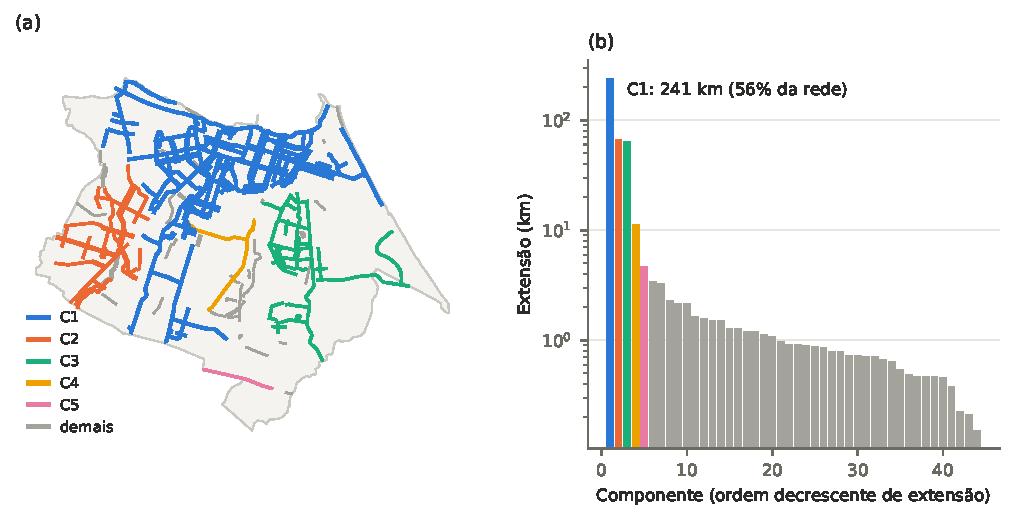
\includegraphics[width=\textwidth]{figuras/conectividade.pdf}
\caption{(a) Ciclovias e ciclofaixas de Fortaleza coloridas pelos cinco maiores componentes conectados (tolerância de 10~m). (b) Extensão de cada componente em ordem decrescente, em escala logarítmica.}
\label{fig:conectividade}
\end{figure}

O resultado varia pouco com a tolerância. Entre 5 e 50~m, o maior componente reúne de 52\% a 57\% da extensão. Sem tolerância e sem considerar cruzamentos, a rede se fragmentaria em 193 componentes, e o maior teria só 23~km. Essa fragmentação é artificial: vem de pontas desenhadas quase encostadas. Na triagem por satélite, 63 das 77 conexões conferidas eram encontros em nível, 11 eram passagens em desnível e 3 ficaram inconclusivas. Apenas uma passagem em desnível era crítica. Cinco delas são cruzamentos da Via Expressa, que permanece ligada à rede pelas extremidades. Retirar também as inconclusivas reduz o maior componente a 55\%.

%==================================
% CONCLUSÃO
%==================================
\section{Conclusão}
A rede de ciclovias e ciclofaixas de Fortaleza não é contínua. Pouco mais da metade da extensão está em um único componente, e duas grandes redes regionais, a oeste e a sudeste, funcionam como ilhas a poucas centenas de metros dele. A extensão total, portanto, superestima a rede efetivamente utilizável sem trechos em tráfego misto. Ligações curtas nos pontos identificados teriam efeito desproporcional sobre a conectividade.

O estudo tem limitações. Uma desconexão na base não impede a circulação de bicicleta pelas vias comuns; indica apenas a falta de infraestrutura dedicada. Um encontro em nível não garante travessia sinalizada, e só 15 das conexões conferidas tinham sinalização cicloviária visível. A base reflete principalmente 2022, e as imagens de satélite não têm data informada. O grafo não direcionado ignora o sentido de circulação das ciclofaixas unidirecionais. Por fim, a análise é estrutural e não mede segurança, conservação nem uso.

%==================================
% REFERÊNCIAS
%==================================
\begin{thebibliography}{99}
\small

\bibitem{bettencourt2021}
  L.~M.~A. Bettencourt.
  \emph{Introduction to Urban Science: Evidence and Theory of Cities as Complex Systems}.
  MIT Press, 2021.

\bibitem{bruno2024}
  M. Bruno, H.~P.~M. Melo, B. Campanelli, V. Loreto.
  A universal framework for inclusive 15-minute cities.
  \emph{Nature Cities}, 1:633--641, 2024.

\bibitem{buehler2016}
  R. Buehler, J. Dill.
  Bikeway networks: a review of effects on cycling.
  \emph{Transport Reviews}, 36(1):9--27, 2016.

\bibitem{fortaleza2024}
  Prefeitura de Fortaleza.
  Malha cicloviária. Portal de Dados Abertos de Fortaleza, 2024.
  Disponível em: \texttt{dados.fortaleza.ce.gov.br}. Acesso em: 19 out. 2026.

\bibitem{hansen1959}
  W.~G. Hansen.
  How accessibility shapes land use.
  \emph{Journal of the American Institute of Planners}, 25(2):73--76, 1959.

\bibitem{maia2023}
  G. Maia, C. Ponte, C. Caminha, L.~S. Furtado, H.~P.~M. Melo, V. Furtado.
  A global empirical study on how street networks facilitate driving longer distances.
  \emph{Scientific Reports}, 13:18154, 2023.

\bibitem{natera2020}
  L.~G. Natera Orozco, F. Battiston, G. Iñiguez, M. Szell.
  Data-driven strategies for optimal bicycle network growth.
  \emph{Royal Society Open Science}, 7:201130, 2020.

\bibitem{opovo2022}
  O Povo.
  Malha cicloviária de Fortaleza ainda é concentrada em bairros centrais.
  Fortaleza, 27 jan. 2022.

\bibitem{szell2022}
  M. Szell, S. Mimar, T. Perlman, G. Ghoshal, R. Sinatra.
  Growing urban bicycle networks.
  \emph{Scientific Reports}, 12:6765, 2022.

\bibitem{xu2020}
  Y. Xu, L.~E. Olmos, S. Abbar, M.~C. González.
  Deconstructing laws of accessibility and facility distribution in cities.
  \emph{Science Advances}, 6(37):eabb4112, 2020.

\end{thebibliography}

\end{document}
